\documentclass[../main.tex]{subfiles}
\begin{document}
\chapter{Theoretical context}
\label{intro:chap:theo}

The Standard Model (SM) of particle physics is a theory that describes the elementary particles and the interactions between them. It provides a set of predictions very well experimentally tested. A brief description of it is given in Section~\ref{theo:sec:sm}. Section~\ref{theo:sec:hh} introduces a description of the phenomenology of the double Higgs production. Finally, Section~\ref{theo:sec:pp} describes the physics of a proton-proton collision and its modelling.

\section{The Standard Model}
\label{theo:sec:sm}

The SM is a gauge invariant and renormalizable quantum field theory (QFT) based on quantum mechanics and special relativity. Elementary particles correspond to excited states of quantum fields. The propagation and interactions of fields in a QFT are fully determined by a Lagrangian density, $\mathcal{L}$, that depends on the fields, $\psi_i$, their derivatives, $\partial_\mu \psi_i$ and the space-time coordinates, $x^\mu$. 


The SM describes the effect of fundamental interactions as a QFT with an exchange of force-mediating particles. This theory shall be invariant under local gauge symmetries, which, by the Noether's theorem, enforces the conservation of charges associated to the interactions. Additionally, imposing the theory to be invariant under these transformations requires introducing additional vector fields, corresponding to the gauge bosons that mediate the interactions. Two interactions are present in the SM: the strong interaction, invariant under $SU(3)_C$, and the electroweak interaction, invariant under $SU(2)_L\times U(1)_Y$.


The Lagrangian $\mathcal{L}$ provides probability amplitudes for the involved physics processes. However, it cannot be solved analytically but requires perturbation theory. The effect of these perturbations can be approximated with expansions in leading-order (LO) or higher orders (next-to-leading-order or NLO, NNLO, and so on). These perturbation terms can be used to build \textit{matrix elements}, which give information about the strength of the process (i.e. its \textit{cross section}) and the kinematics of the final state particles. They are often illustrated as Feynman diagrams.

The particle content of the Standard Model is shown in Fig.~\ref{theo:fig:sm}. Two types of particles are included in the SM: matter particles, fermions with spin~$=1/2$ associated to fields represented by spinors, and bosons with spin~$=1$, associated to vectorial fields, that mediate the interactions between fermions. Additionally, the Higgs boson, associated to a scalar field, is included as a mechanism to give masses to both fermions and bosons.

\begin{figure}[h!]
\begin{center}
of 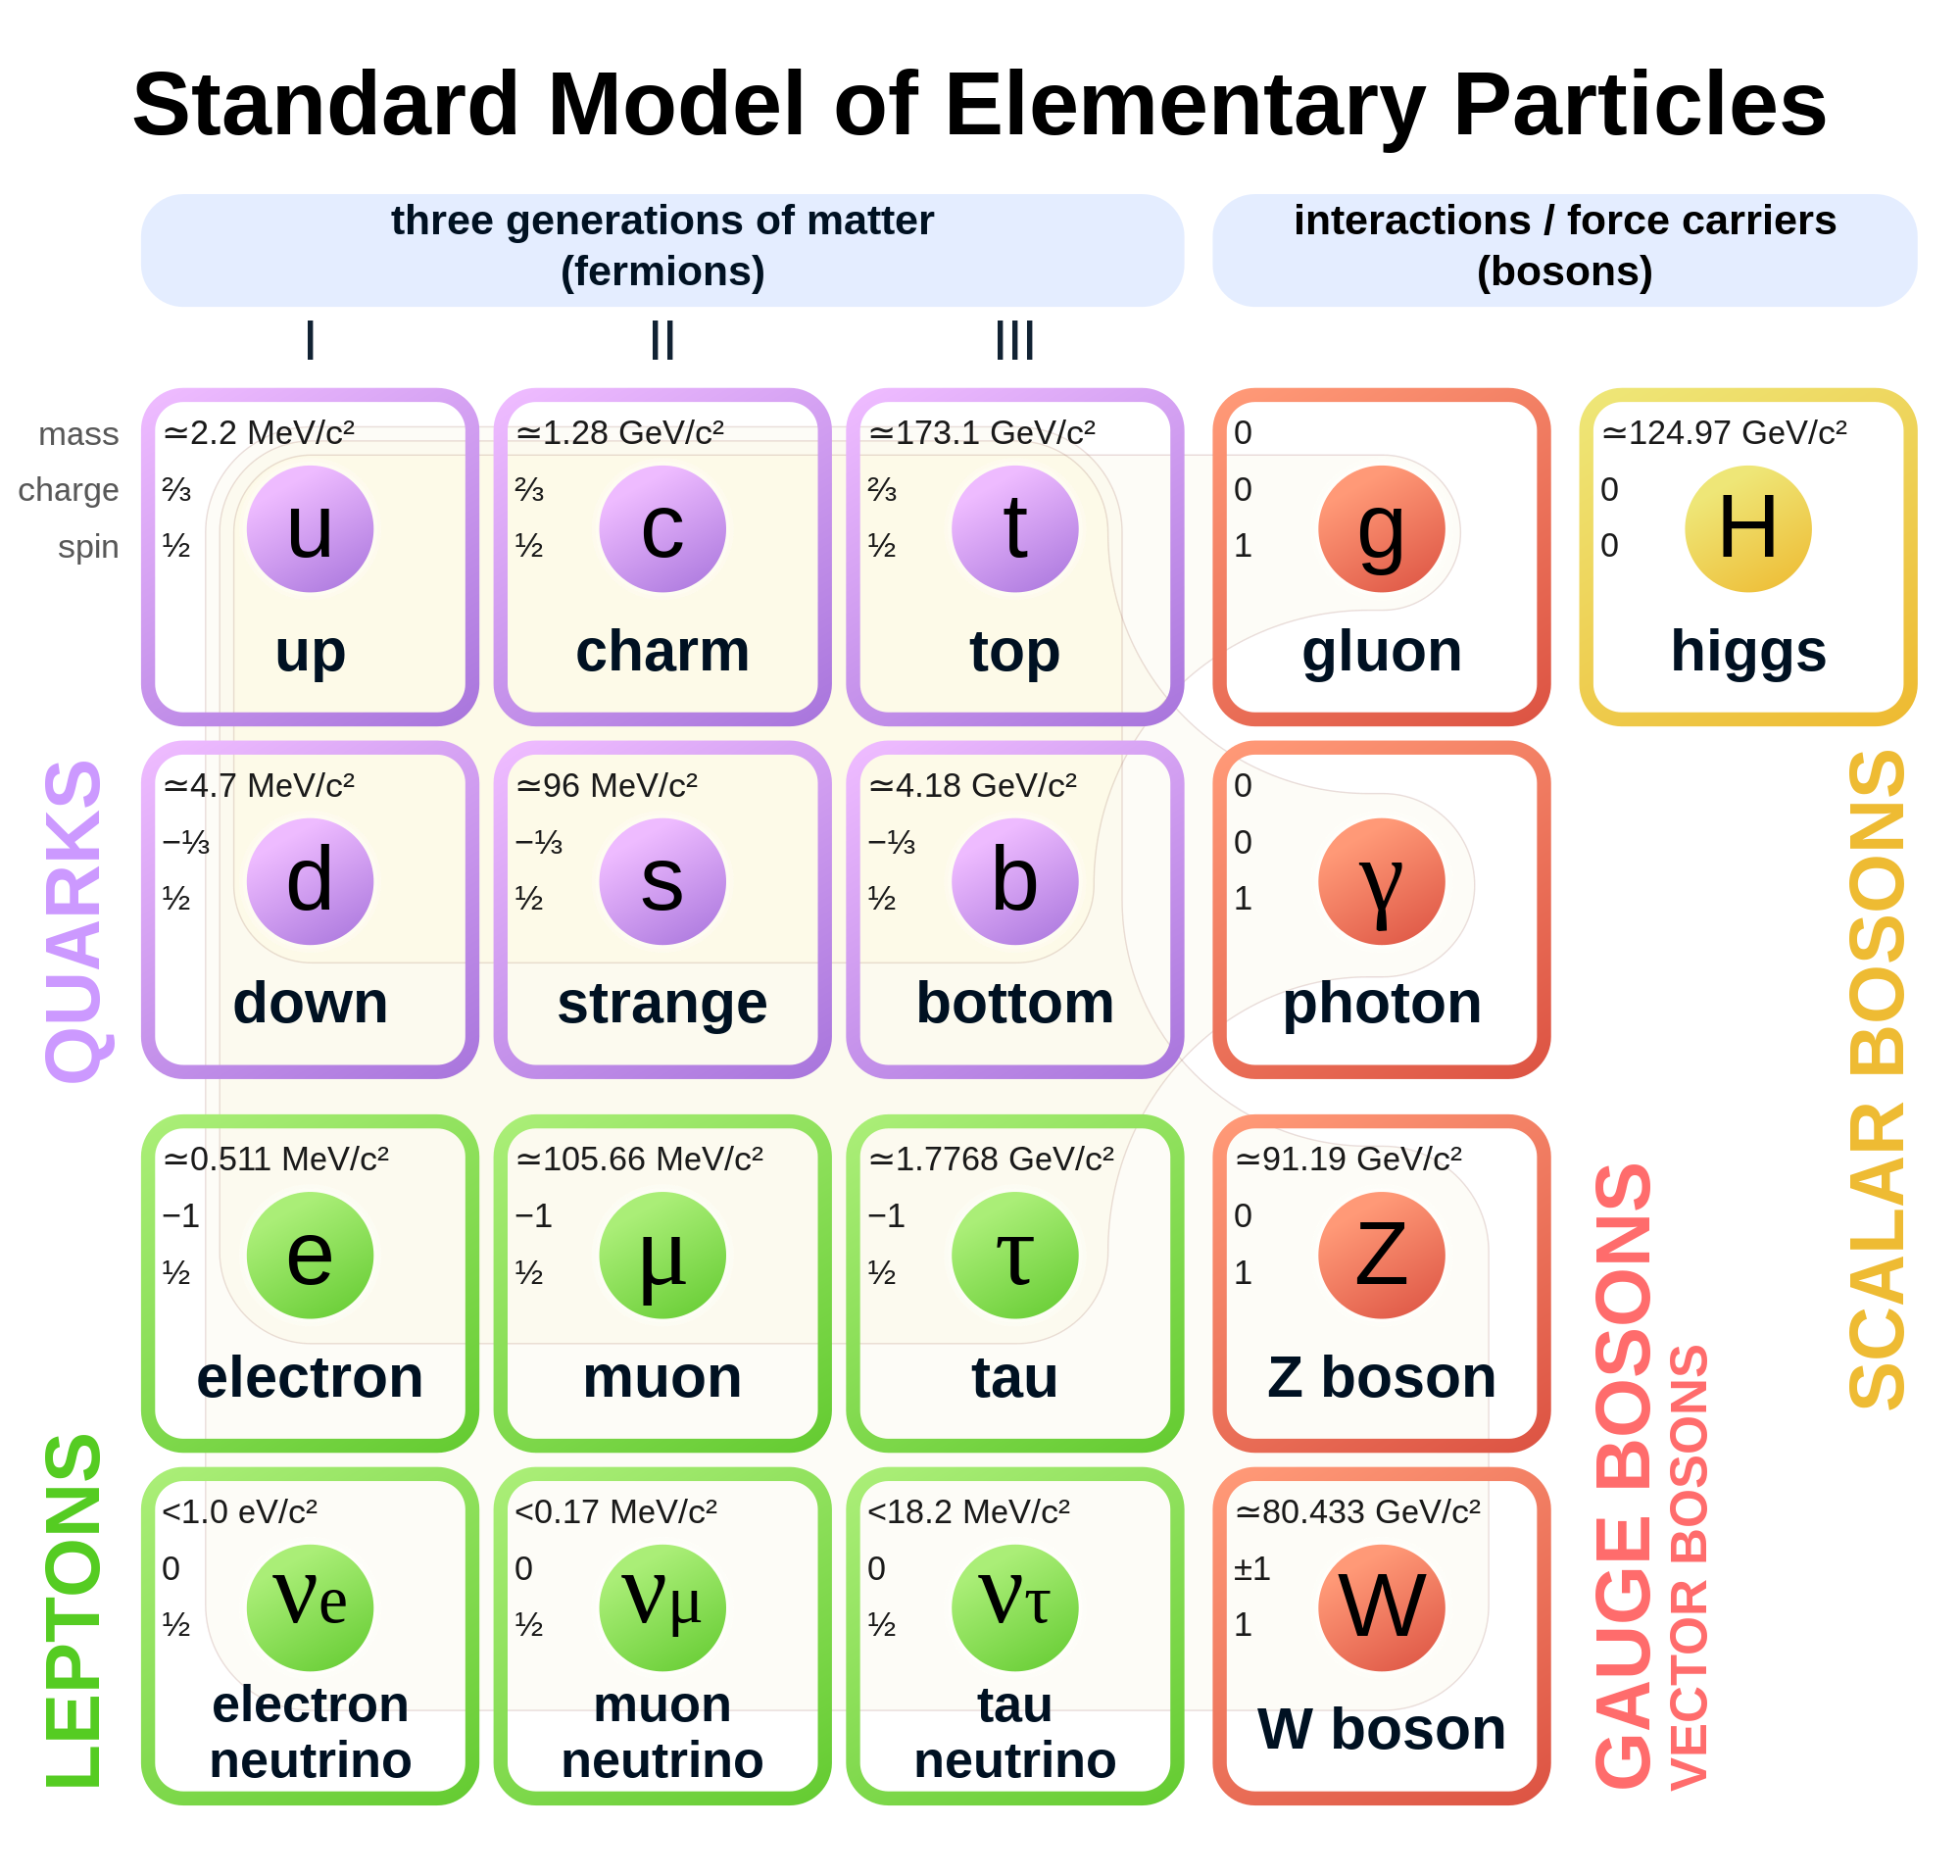
\includegraphics[width=0.6\textwidth]{Images/Standard_Model_of_Elementary_Particles}
\end{center}
\caption[Particle content of the Standard Model of particle physics]{Particle content of the Standard Model of particle physics. Extracted from \cite{intro:theo:sm_pic}. }
\label{theo:fig:sm}
\end{figure}

Even if the SM has been a very successful theory, explaining most of the experimental results with a very high level of accuracy, it does not provide a complete understanding of Nature. In particular, it is challenged by the existence of dark matter, the asymmetry in the Universe between matter and antimatter, or even the values of the fundamental parameters of the SM itself. The SM is clearly incomplete, and must be taken as an effective theory valid in a particular energy (or mass) range. The theories that extend the Standard Model in order to include explanations about these known problems are referred to as \textit{Beyond the Standard Model} (BSM) theories. Some examples of them are theories based on supersymmetry, such as the Minimal Supersymmetric Standard Model (MSSM) and Next-to-Minimal Supersymmetric Standard Model (NMSSM), string theory, or extra dimensions.




\subsection{Matter particles}

Twelve fermions have been experimentally observed and are described in the SM, six \textit{quarks} and six \textit{leptons}. Both quarks and leptons are divided in three \textit{generations}, each containing two quarks with electric charges $Q=+2/3$ and $-1/3$, and two leptons with $Q=-1$ and $0$. Each fermion has its corresponding \textit{antiparticle}, with the same characteristics but opposite quantum numbers, including the electric charge. Quarks are the only particles in the SM affected by the three forces, the electromagnetic, the weak, and the strong forces, described in the next sections. 

The first generation of quarks is composed by the \textit{up} (u) and \textit{down} (d) quarks, with masses of 2.2~MeV and 4.7~MeV \cite{pdg}, respectively. The second generation, the \textit{charm} (c) and \textit{strange} (s) quarks, have masses of 1.27~GeV and 93.4~MeV \cite{pdg}, respectively. The \textit{top} (t) and \textit{bottom} (b) quarks form the third generation, with masses of 172.7~GeV and 4.18~GeV. Each quark carries a \textit{flavour} and a \textit{colour}, which makes them subject to the electroweak and the strong forces, respectively. A property of the strong force is the \textit{color confinement}, which implies that quarks cannot exist as free states, but are experimentally observed as bound states called \textit{hadrons}. The top quark, however, cannot form hadrons, since its very high mass makes it very unstable, decaying right after being produced. At higher energies, the strong force gets increasingly weaker, so quarks behave like \textit{asymptotically free} particles. This allows to study their interactions in proton colliders like the LHC.


\textit{Electrons} (e), \textit{muons} ($\mu$) and \textit{taus} ($\tau$) are the three charged leptons included in the SM, with masses of 0.511~MeV, 105.66~MeV and 1.78~GeV respectively \cite{pdg}. These particles are subject to the electromagnetic and the weak forces. The electron is the only stable charged lepton. Muons have a lifetime of 2.2~$\mu$s \cite{pdg}, nonetheless they are still detectable by collider experiments thanks to their high momentum and the experiment size. Tau leptons, however, have a lifetime of 290.3~fs, so they decay before being detected and can only be inferred from its decay products.

Each charged lepton is associated to a electrically neutral neutrino of the same flavour ($\nu_e$, $\nu_\mu$ and $\nu_\tau$). In the classical SM formulation, these neutrinos are massless. However, the observation of neutrino flavour oscillations \cite{intro:theo:nu_oscillations} implies that neutrinos are massive, with upper limits on their masses of $m(\nu_e)<1.1$~eV, $m(\nu_\mu)<0.19$~MeV, and $m(\nu_\tau)<18.2$~MeV \cite{pdg}. Neutrinos only interact with matter via the weak force, so they can not be directly detected at collider experiments. Their presence is reconstructed from the energy imbalance in the event (see Section~\ref{intro:subsec:met}).

\subsection{Interactions in the Standard Model}

\subsubsection{The strong interaction}

The strong interaction is described by the Quantum Chromodynamics (QCD) theory. QCD is a non-abelian gauge theory based on the $SU(3)_C$ group. The conserved charge associated to this symmetry is the color charge. As only quarks have color charge, only quark fields have a fundamental representation under this group; the other fermions have the trivial representation. The $SU(3)_C$ group has eight generators, $T^a$, the Gell-Mann matrices, related to the eight \textit{gluons}, the massless strong force mediators. The QCD Lagrangian can be written as
\begin{equation}
\mathcal{L}_{\text{QCD}} = \bar{\psi}\left(i\gamma^\mu\partial_\mu - g_s\gamma^\mu T_a G^a_\mu - m\right)\psi - \frac{1}{4}G_{\mu\nu}^a G_a^{\mu\nu},
\end{equation}
where $\gamma^\mu$ are the Dirac matrices,  $\psi$ is the quark field, $m$ is the quark mass, $g_s$ is the coupling constant of the strong interaction (although $\alpha_s = \frac{g_s^2}{4\pi}$ is more commonly used) and the strength field tensor $G_{\mu\nu}^a$ is defined as 
\begin{equation}
G_{\mu\nu}^a = \partial_\mu G_\nu^a - \partial_\nu G_\mu^a - g_s f^{abc} G_\mu^b G_\nu^c,
\end{equation}
where $f^{abc}$ are the structure constants of the $SU(3)_C$ group. The last term of the strength field tensor is included since the $SU(3)_C$ is non-abelian. This term leads to 3- and 4-gluons self-interactions.

\subsubsection{The electroweak interaction}

The electroweak (EWK) interaction is a unified description of the electromagnetic and weak interactions. It's a theory locally gauge invariant under $SU(2)_L \times U(1)_Y$ transformations.

The weak interaction is a theory described with the non-abelian $SU(2)_L$ group. It has the peculiarity that it violates parity, i.e.~left and right-handed particles couple differently. The concept of \textit{chirality} is then introduced in the theory: the chirality is a Lorentz-invariant quantity corresponding to the eigenvalues of $\gamma^5=i\gamma^0\gamma^1\gamma^2\gamma^3$ ($\pm1$), giving rise to the left ($\psi_L$) and right ($\psi_R$) chirality fields, obtained as
\begin{align}
\label{theo:eq:chiral_1}
\psi_L &= \frac{1}{2}(1 - \gamma^5)~\psi, \\
\label{theo:eq:chiral_2}
\psi_R &= \frac{1}{2}(1 + \gamma^5)~\psi.
\end{align}

Every fermionic field of the SM is represented as one left chirality doublet ($\psi_L$) and two right chirality singlets ($\psi_R$, $\psi'_R$). For example, for the first family of quarks
\begin{equation}
\psi_L = \left(
\begin{matrix}
u_L \\
d_L
\end{matrix}
\right), \psi_R = u_R, \psi'_R = d_R,
\end{equation}
and, similarly, for the first family of leptons
\begin{equation}
\label{theo:eq:ele_chiral}
\psi_L = \left(
\begin{matrix}
\nu_{e, L} \\
e_L
\end{matrix}
\right), \psi_R = \nu_{e,R}, \psi'_R = e_R.
\end{equation}

The conserved charge associated to the $SU(2)_L$ group is the \textit{weak isospin} $I_3$. For left-handed fermions, the up-type takes a value of $I_3=+1/2$ and the down-type $I_3=-1/2$. Right-handed fermions, as they are singlets of $SU(2)_L$, take a value of $I_3=0$.

The weak Lagrangian can be written as
\begin{equation}
\mathcal{L}_{\text{WK}} = i\bar{\psi}_L\gamma_\mu D_\mu \psi_L + i \bar{\psi}_R\gamma^\mu\partial_\mu\psi_R + i \bar{\psi}'_R\gamma^\mu\partial_\mu\psi'_R - \frac{1}{4}W_{\mu\nu}^i W_i^{\mu\nu},
\end{equation}
where
\begin{equation}
D_\mu = \partial_\mu + ig_w T^i W_\mu^i
\end{equation}
is the covariant derivative of the $SU(2)_L$ group with $i\in\{1, 2, 3\}$, $g_w$ is the coupling constant of the weak force, $W_\mu^i$ are the three gauge fields, $T_\mu^i = \sigma_i / 2$ ($\sigma_i\equiv$~Pauli matrices) are the generators of $SU(2)_L$ and the tensor field $W_{\mu\nu}^i$ is defined as
\begin{equation}
\label{theo:eq:wmunu}
W_{\mu\nu}^i = \partial_\mu W_\nu^i - \partial_\nu W_\mu^i - g_w \epsilon_{ijk}W_\mu^j W_\nu^k,
\end{equation}
where $\epsilon_{ijk}$ are the structure constants of $SU(2)_L$. The last term of Eq.~\eqref{theo:eq:wmunu} adds interaction terms between three and four gauge fields. Note that a mass term $m\bar{\psi}\psi = m(\bar{\psi}_R\psi_L + \bar{\psi}_L \psi_R)$ has not been added to the Lagragian, as it's not invariant under $SU(2)_L$.

The gauge fields $W_\mu^i$ do not correspond to the physical $W_\mu^\pm$ and $Z_\mu$ fields associated to the W${}^\pm$ and Z bosons. The first ones can be obtained via a linear combination
\begin{equation}
\label{theo:eq:w}
W_\mu^\pm = \frac{1}{\sqrt{2}}(W_\mu^1 \mp i W_\mu^2).
\end{equation}

To obtain the $Z_\mu$ boson field, an additional group $U(1)_Y$ inspired in the electromagnetic theory is introduced, with a Lagrangian
\begin{equation}
\mathcal{L}_\text{Y} = i\bar{\psi}\gamma^\mu D_\mu \psi - \frac{1}{4}B_{\mu\nu}B^{\mu\nu},
\end{equation}
where
\begin{equation}
D_\mu = \partial_\mu + ig_Y Y B_\mu
\end{equation}
is the covariant derivative of $U(1)_Y$, $g_Y$ is the coupling constant and the tensor field $B_{\mu\nu}$ is defined as
\begin{equation}
B_{\mu\nu} = \partial_\mu B_\nu - \partial_\nu B_\mu.
\end{equation}

The conserved quantity of this symmetry is the hypercharge, $Y$, related to the isospin and the electric charge by $Y = 2 (Q - I_3)$. With this additional field, the Z boson and the photon ($\gamma$) fields $Z_\mu$ and $A_\mu$ can be obtained as
\begin{equation}
\label{theo:eq:az}
\left(
\begin{matrix}
Z_\mu \\
A_\mu
\end{matrix}
\right)
=
\left(
\begin{matrix}
\cos \theta_W & - \sin \theta_W \\
\sin \theta_W &   \cos \theta_W
\end{matrix}
\right)
\left(
\begin{matrix}
W^3_\mu \\
B_\mu
\end{matrix}
\right),
\end{equation}
where $\theta_W$ is the Weinberg angle, defined as
\begin{equation}
\theta_W = \tan^{-1} \frac{g_W}{g_Y}.
\end{equation}

Up to this point, the $W^\pm$, Z and $\gamma$ bosons and the fermions have been assumed to be massless, since typical mass terms would break the gauge invariance. However, experimentally all those particles have been measured as massive particles (with the exception of the photon). The mechanism through which fermions and bosons acquire mass comes from the spontaneous symmetry breaking of the electroweak symmetry, described below.

\subsection{The electroweak symmetry breaking}
\label{theo:subsec:ewsb}

Since the EWK bosons are not massless, additional terms need to be introduced in the Lagragian by breaking the electroweak symmetry without breaking the gauge invariance. These mass terms arise from the so-called electroweak symmetry breaking (EWSB).

In the SM, the EWSB is achieved through the \textit{Higgs mechanism}, proposed in 1964 independently by P. Higgs \cite{intro:theo:peter_higgs} and F. Englert and R. Brout \cite{intro:theo:englert_brout}, among others. This mechanism explains the masses of gauge bosons and fermions by proposing that the $SU(2)_L\times U(1)_Y$ symmetry from the EWK theory is broken at low energies and becomes $U(1)_{EM}$. This symmetry breaking is based on the introduction of two new complex scalar fields grouped in a weak isospin doublet $\phi$ known as the Higgs field:
\begin{equation}
\phi = 
\left(
\begin{matrix}
\phi^+ \\
\phi^0
\end{matrix}
\right)
= 
\frac{1}{\sqrt{2}}
\left(
\begin{matrix}
\phi_1 + i\phi_2 \\
\phi_3 + i\phi_4 
\end{matrix}
\right),
\end{equation}
where $\phi_1$, $\phi_2$, $\phi_3$ and $\phi_4$ are real scalar fields. The Lagrangian associated to this field can be written as
\begin{equation}
\label{theo:eq:higgs_lagrangian}
\mathcal{L}_{\text{Higgs}} = (D_\mu\phi)^\dag (D_\mu\phi) - V(\phi),
\end{equation}
where $D_\mu$ is the covariant derivative from the EWK theory
\begin{equation}
D_\mu = \partial_\mu + ig_w T^i W_\mu^i + i g_Y Y B_\mu
\end{equation}
and $V(\phi)$ is a potential that has the form
\begin{equation}
V(\phi) = \mu^2\phi^\dag\phi + \lambda(\phi^\dagger\phi)^2,
\end{equation}
where $\mu^2$ and $\lambda$ are constants. In the case where $\mu^2>0$ and $\lambda>0$, the potential will have a parabolic shape with a minimum in $\phi=0$, i.e.~the corresponding to a scalar particle with mass $\mu$ and self-interaction with a coupling $\lambda$. However, if $\mu^2<0$, the shape of the potential is illustrated in Fig.~\ref{theo:fig:higgs_potential}, the so-called \textit{mexican hat} shape. In this case, $\phi=0$ becomes a local maximum, and the minima are found in the doublets that satisfy
\begin{equation}
\phi^\dagger\phi = \frac{-\mu^2}{2\lambda} \equiv \frac{v^2}{2},
\end{equation}
where $v$ is the \textit{vacuum expectation value}. Among all possible states, the ground state can be expressed, without loss of generality, as
\begin{equation}
\phi_\text{ground} = \frac{1}{\sqrt{2}}\left(
\begin{matrix}
0 \\
v
\end{matrix}
\right)
\end{equation}

\begin{figure}[h!]
\begin{center}
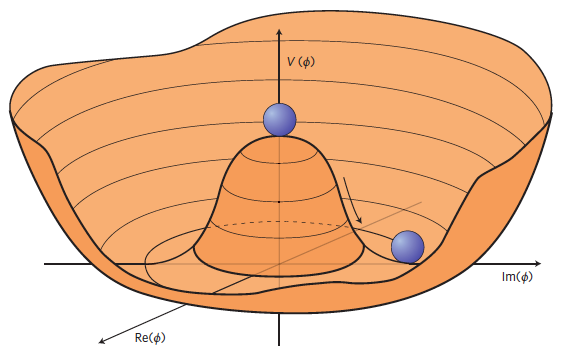
\includegraphics[width=0.5\textwidth]{Images/higgspotential}
\end{center}
\caption[Higgs potential in the case that $\mu^2 < 0$]{Illustration of the Higgs potential in the case that $\mu^2 < 0$. Extracted from \cite{intro:theo:higgs_potential_picture}.}
\label{theo:fig:higgs_potential}
\end{figure}

By exciting around the ground state, $\phi(x)$ becomes
\begin{equation}
\label{theo:eq:higgs_field}
\phi(x) = \frac{1}{\sqrt{2}}
\left(
\begin{matrix}
0 \\
v + H(x)
\end{matrix}
\right),
\end{equation}
where $H(x)$ is the only field that remains, the one associated to a new massive particle, the Higgs boson (H).

By including Eq.~\ref{theo:eq:higgs_field} and the transformations shown in Eqs.~\ref{theo:eq:w} and \ref{theo:eq:az} into the Lagrangian from Eq.~\ref{theo:eq:higgs_lagrangian}, the Lagrangian can be rewritten as
\begin{align}
\label{theo:eq:boson_masses}
\mathcal{L}_{\text{Higgs}} &= \frac{1}{2}\partial_\mu H \partial^\mu H + \frac{g_w^2 v^2}{4}W_\mu^+ W^{-\mu} + \frac{1}{2}\frac{g_w^2 + g_Y^2}{4}v^2 Z_\mu Z^\mu + \frac{1}{2}2\mu^2H^2 \\
\label{theo:eq:vvh}
&+ \frac{g_w^2}{2}vHW_\mu^+W^{-\mu} + \frac{g_Y^2}{2}vHZ_\mu Z^\mu\\
\label{theo:eq:vvhh}
&+ \frac{g_w^4}{2}H^2W_\mu^+W^{-\mu} + \frac{g_Y^2}{4}H^2Z_\mu Z^\mu\\
\label{theo:eq:hh}
&+ \frac{\mu^2}{v}H^3 + \frac{\mu^2}{4\nu^2}H^4.
\end{align}

The second, third, and fourth terms of Eq.~\eqref{theo:eq:boson_masses} correspond to mass terms for the W${}^\pm$, Z, and H bosons, so these bosons acquire masses given by
\begin{equation}
M_\text{Z} = \frac{\sqrt{g_w^2 + g_Y^2}}{2}v , \qquad M_{\text{W}^\pm}= \frac{g_w v}{2} = M_Z \cos \theta_W, \qquad M_\text{H} = \sqrt{2}\mu.
\end{equation}

No mass term appears for the $A_\mu$ field, so the photon remains massless.

The rest of the terms in the Lagrangian are interaction terms. Eqs.~\eqref{theo:eq:vvh} and \eqref{theo:eq:vvhh} include trilinear HZZ and HW${}^+$W${}^-$ and quadrilinear HHZZ and HHW
${}^+$W${}^-$ couplings. Eq.~\eqref{theo:eq:hh} includes the trilinear and quadrilinear Higgs boson self-interactions HHH and HHHH. With these terms, the Higgs \textit{self-couplings} can be defined as
\begin{equation}
\lambda_{\text{HHH}} = \lambda_{\text{HHHH}} = \frac{M_H^2}{2v^2} \equiv \lambda.
\end{equation}

The presence of these interaction terms shows that the double (and triple) Higgs production is predicted by the SM at tree level. Studying this production is an important test of the electroweak symmetry breaking.

Finally, the mass of the fermions also raises from their interactions with the Higgs field. For a given fermionic field, using its chirality components (obtained via Eqs.~\eqref{theo:eq:chiral_1} and \eqref{theo:eq:chiral_2}), one can write its interaction with the Higgs field with a Yukawa Lagrangian:
\begin{equation}
\mathcal{L}_{\text{Yukawa}} = -y_F(\bar{\psi}_R\phi^\dagger\psi_L + \bar{\psi}_L\phi\psi_R),
\end{equation}
where $y_F$ is the coupling constant between the fermion and the Higgs boson. As an example, for the electron field shown in Eq.~\eqref{theo:eq:ele_chiral}, by introducing $\phi$ parametrized as in Eq.~\eqref{theo:eq:higgs_field}, one obtains:
\begin{equation}
\label{theo:eq:ele_lag_1}
\mathcal{L}_{\text{Yukawa}, e} = -y_e \frac{v + H}{\sqrt{2}}(\bar{e}_R e_L + \bar{e}_L e_R).
\end{equation}

By re-grouping the electron fields as $\bar{e} = (\bar{e}_R,\bar{e}_L)$ and $e = (e_R, e_L)$, Eq.~\eqref{theo:eq:ele_lag_1} becomes
\begin{equation}
\label{theo:eq:ele_lag_2}
\mathcal{L}_{\text{Yukawa}, e} = -y_e \frac{v}{\sqrt{2}} \bar{e}e -y_e \frac{H}{\sqrt{2}} \bar{e}e.
\end{equation}

The first term in Eq.~\eqref{theo:eq:ele_lag_2} corresponds to the mass term of the electron field, so the mass of the electron can be obtained as $m_e = \frac{y_e v}{\sqrt{2}}$. The second term represents the interaction between the Higgs boson and the electron.

In conclusion, the EWSB allows both fermions and bosons to acquire mass via the Higgs field. All masses and interactions between the Higgs boson and the particles are related to $v$ and the gauge couplings. In fact, the interactions between the Higgs boson and the particles are proportional to masses of the latter, so the Higgs boson will decay preferentially to the heaviest particles kinematically accesible.

\subsection{Phenomenology of the Higgs boson}

On July 4 2012, the CMS and ATLAS experiments at the LHC at CERN announced the observation of a new boson compatible with the SM prediction of the Higgs boson \cite{intro:theo:cms_higgs, intro:theo:atlas_higgs}. The discovery was performed independently by the two experiments using data from the first two years of the LHC Run 1 (2011-2012, see Section~\ref{intro:sec:lhc}).

Regarding the mass of the Higgs boson, the most recent and precise value was obtained by combining the results from the CMS experiment during 2011, 2012 and 2016 at centre-of-mass energies of $\sqrt{s}=7,~8$~and~$13$~TeV, respectively \cite{intro:theo:cms_higgs_mass}. The resulting value was
\begin{equation}
m_\text{H} = 125.38 \pm 0.11 ~(\text{stat}) \pm 0.08 ~(\text{syst}) ~\text{GeV}.
\end{equation}

The SM predicts that the Higgs boson is a electrically neutral scalar particle (spin$~=0$) and even under charge conjugation parity (CP) transformations. Both properties have been determined. Due to the Landau-Yang theorem, the observation of the Higgs boson decaying into $\gamma\gamma$ forbids it to have a spin$~=1$ \cite{intro:theory:landau, intro:theory:yang}. The spin-0 vs spin-2 and the CP hypotheses have been studied using the Higgs boson decay into two Z bosons \cite{intro:theory:cmshzz}, confirming the SM prediction.

Once the Higgs boson mass has been measured, its production modes and their cross sections can also be studied. Fig.~\ref{theo:fig:h_production_xs} shows the Higgs boson main production modes cross sections for a Higgs boson mass of 125~GeV as a function of the collision centre-of-mass energy. The dominant production mode is gluon fusion (ggF), where the Higgs boson is produced via loops of heavy quarks (mostly t quarks); its cross section is around 49~pb at $\sqrt{s}=13$~TeV. The production mode with the second largest contribution is vector boson fusion (VBF), where the Higgs boson is produced in association with two high-momentum quarks very close to the direction of the incident particles. Its cross section is about 10 times smaller than ggF, 3.8~fb. Follows the associated production with a vector boson, with a cross section of 2.3~pb, and the associated production with heavy quarks (top pair, bottom pair or single top), with cross sections around one order of magnitude smaller than the previous. The Feynman diagrams of these processes are shown in Fig~\ref{theo:fig:h_feynman}.

\begin{figure}[h!]
\begin{center}
\includegraphics[width=0.6\textwidth]{Images/hxs}
\end{center}
\caption[SM Higgs boson production cross sections]{The SM Higgs boson production cross sections as a function of the LHC centre of mass energy for a Higgs boson mass of 125~GeV. The main production modes at the LHC are shown: gluon fusion (blue), vector boson fusion (red), vector boson associated production (green and black), top quark pair associated production (dark purple), bottom quark pair associated production (pink) and single top associated production (light purple). Extracted from \cite{intro:theo:yellow_higgs}.}
\label{theo:fig:h_production_xs}
\end{figure}

\begin{figure}[h!]
\begin{center}
\includegraphics[trim = 0 159 0 0, width=0.8\textwidth]{Images/hprod}
\end{center}
\caption[LO Feynman diagrams of the main Higgs boson production modes]{Leading-order Feynman diagrams of the main Higgs boson production modes at the LHC.}
\label{theo:fig:h_feynman}
\end{figure}

The \textit{branching fractions} or \textit{branching ratios} (BR) of the Higgs boson (i.e.~the probability of the Higgs boson decaying into different final states) for a mass of 125~GeV are shown in Table~\ref{theo:tab:h_br}. The decay with the largest BR is the H~$\to$~bb, with a BR of 58\%. However, this channel is not the most appropriate to perform experimental studies at the LHC, as other processes with similar final states are very commonly produced from pp collisions. Instead, the most convenient final states are the H~$\to\gamma\gamma$ and H~$\to$~ZZ~$\to4l$ ($l=e,~\mu$), as the detector resolutions on the objects from  these final states are very high.

\begin{table}[h!]
\begin{center}
\begin{tabular}{c | c}
Decay channel & BR (\%) \\\hline
bb & 58.24 \\
WW & 21.37 \\
gg & 8.187 \\
$\tau\tau$ & 6.272 \\
c$\bar{\text{c}}$ & 2.891 \\
ZZ & 2.619 \\
$\gamma\gamma$ & 0.227
\end{tabular}
\caption[Higgs decay branching fractions]{Branching fractions (in \%) for the H decay into the most probable final states for a Higgs boson mass of 125~GeV. Values extracted from \cite{intro:theo:yellow_higgs}.}
\label{theo:tab:h_br}
\end{center}
\end{table}

After having experimentally established the Higgs boson production and its decay modes, the linear proportionality between the Higgs boson couplings and the mass of the fermions, and the squared proportionality with respect to the mass of the vector bosons can be verified. As shown in Fig.~\ref{theo:fig:h_coupling_masses}, the measured couplings with fermions and vector bosons follow the predicted dependency on the mass of the particles for a wide range of particle masses, which gives a strong evidence of the validity of the EWSB mechanism.

\begin{figure}[h!]
\begin{center}
\includegraphics[width=0.6\textwidth]{Images/h_coupling_masses}
\end{center}
\caption[Normalised coupling constants of the Higgs boson to fermions and vector bosons]{Measured normalised coupling constants of the Higgs boson to fermions and vector bosons, as functions of the fermion or vector boson mass. Extracted from \cite{hh:analysis:nature}.}
\label{theo:fig:h_coupling_masses}
\end{figure}

\section{Higgs boson pair production at the LHC}
\label{theo:sec:hh}

The production of Higgs boson pairs (HH) is a rare process (around 1000 times less probable than single Higgs boson production) predicted by the SM. Its study provides information not only about the Higgs self-coupling, but also about other couplings with the t quark or vector bosons. Precise measurements of these couplings can also probe Beyond the Standard Model (BSM) effects: small variations of their values can lead to big changes in the HH production cross section and the kinematics of the produced particles.

\subsection{HH production modes}

Fig.~\ref{theo:fig:hh_production_xs} shows the cross section for the six main HH production modes and their dependence with respect to the energy of the collision. At 13~TeV (collision energy during the Run 2 of the LHC, see Section~\ref{intro:sec:lhc}), the two dominant production modes are gluon fusion and vector boson fusion. Both are described in the following.


\begin{figure}[h!]
\begin{center}
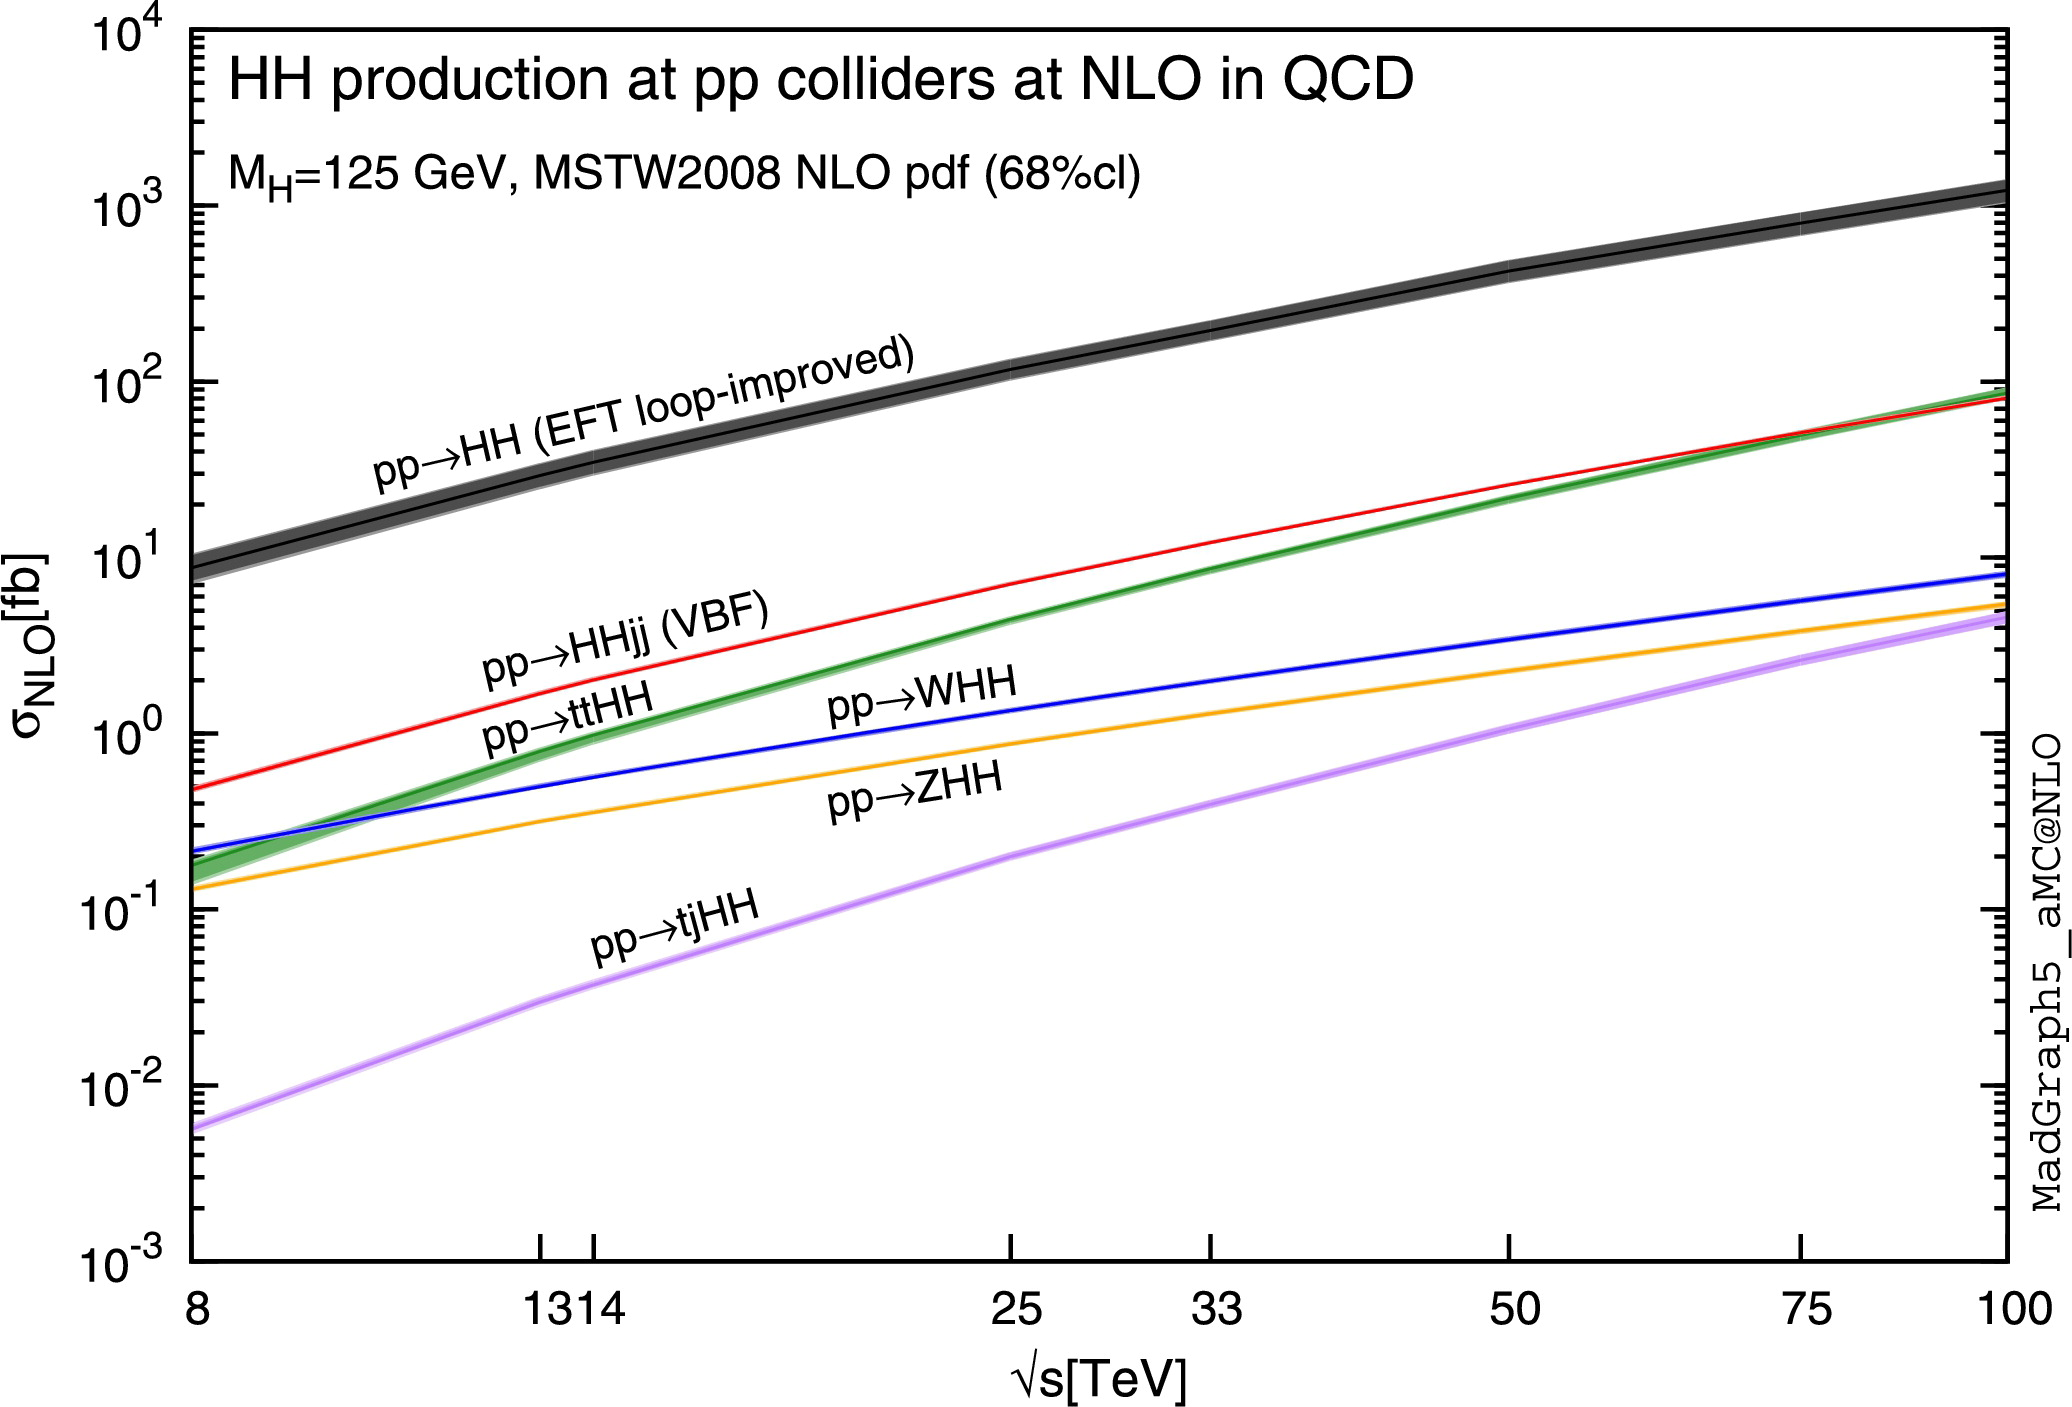
\includegraphics[width=0.6\textwidth]{Images/hh_production_xs}
\end{center}
\caption[Total cross section at NLO for the six largest HH production modes]{Total cross section at NLO for the six largest HH production modes at pp colliders: gluon fusion (black), vector boson fusion (red), top quark pair associated production (green), vector boson associated production (blue and yellow) and single top quark associated production (purple). The thickness of the lines corresponds to the scale and PDF uncertainties (see Section~\ref{theo:sec:pp}). Extracted from \cite{intro:theo:hh_prod_modes}.}
\label{theo:fig:hh_production_xs}
\end{figure}


Gluon fusion (ggF) is the dominant production mode, with a cross section predicted by the Standard Model of around 31~fb. Since gluons are massless, they do not couple to the Higgs boson directly, but through heavy quark loops. This loop is dominated by the t quark ($\sim99\%$), followed by the b quark with 1\%. The LO diagrams of this production mode are shown in Fig.~\ref{theo:fig:ggf_feynman}, denoted as \textit{triangle} and \textit{box} diagrams. The triangle contribution depends linearly on the Higgs boson self-coupling $\lambda$ and the Yukawa coupling $y_t$, while the box diagram only depends quadratically on $y_t$.


\begin{figure}[h!]
\begin{center}
\subfloat{\includegraphics[trim = 0 601 0 0, width=0.45\textwidth]{Images/ggf_triang}}
\subfloat{\includegraphics[trim = 0 590 0 0, width=0.45\textwidth]{Images/ggf_box}}
\end{center}
\caption[HH gluon fusion Feynman diagrams]{Feynman diagrams contributing to Higgs boson pair production via gluon fusion in the SM at leading order. The left diagram is often referred as the \textit{triangle} diagram, whereas the right one, as the \textit{box} diagram.}
\label{theo:fig:ggf_feynman}
\end{figure}

Vector boson fusion (VBF) is the subdominant production mode at the LHC energy ranges, with a cross section predicted in the Standard Model of $\sim1.7$~fb. The most distinctive feature of this production mode is the presence of two additional quarks with high energy and very close to the initial direction of the colliding particles. Experimentally, this translates into a couple of particle jets with high invariant mass and large separation in pseudorapidity (see Section~\ref{intro:sec:lhc}). This effect can be seen in Fig.~\ref{theo:fig:genjj}, showing the distributions of the invariant mass of the two jets with the largest invariant mass, and the difference in pseudorapidity between the two jets with the highest difference, for samples produced via ggF and VBF. Three Feynman diagrams, shown in Fig.~\ref{theo:fig:vbf_feynman}, contribute at LO to this production mode. The first diagram depends linearly on the coupling between two vector bosons and two Higgs bosons, $\lambda_{2V}$. The second depends quadratically on the coupling between two vector bosons and one Higgs boson ($\lambda_{V}$), while the third one linearly on both $\lambda_{V}$ and the Higgs boson self-coupling.

\begin{figure}[h!]
\begin{center}
\subfloat{\includegraphics[width=0.49\textwidth]{Images/max_genjj_mass__noweights__pg_signal__nodata}}
\subfloat{\includegraphics[width=0.49\textwidth]{Images/max_genjj_delta_eta__noweights__pg_signal__nodata}}
\end{center}
\caption[Jet-jet invariant mass and difference in pseudorapidity]{(Left) Invariant mass of the two jets at generator level with the highest invariant mass and (right) difference in pseudorapidity between the two jets at generator level with the highest difference in pseudorapidity, for HH samples produced via VBF (black) and ggF (red).}
\label{theo:fig:genjj}
\end{figure}

\begin{figure}[h!]
\begin{center}
\includegraphics[trim = 0 688 0 0, width=\textwidth]{Images/vbf_1}
\end{center}
\caption[HH vector boson fusion diagrams]{Feynman diagrams contributing to Higgs boson pair production via vector boson fusion in the SM at leading order.}
\label{theo:fig:vbf_feynman}
\end{figure}

Within each production mode, the final cross section is the result of the interference of its corresponding diagrams. For instance, the differential cross section corresponding to the diagrams related to the ggF production mode and their interference is represented in Fig.~\ref{theo:fig:ggf_mass_dependence} as a function of the Higgs pair invariant mass. Its interference is shown to be destructive, which reduces the cross section of this process.


\begin{figure}[h!]
\begin{center}
\includegraphics[width=0.8\textwidth]{Images/ggf_mass_dependence}
\end{center}
\caption[Gluon fusion differential cross section]{Differential cross section corresponding to the different contributions to the gluon fusion production mechanism and their interference. Extracted from \cite{intro:theo:higgs_potential}.}
\label{theo:fig:ggf_mass_dependence}
\end{figure}

The value of the $\lambda$ coupling only depends in the SM on the values of $v$ and $m_H$. However, some BSM theories predict a modification of the $\lambda$ value, varying the properties of the Higgs boson pair production. To study possible BSM effects, a parametric approach is followed, so $\lambda$ is left as a free parameter and deviations from the SM are measured by studying the Higgs self-coupling modifier, defined as
\begin{equation}
\kappa_\lambda = \lambda / \lambda_{\text{SM}}.
\end{equation}

Changes on the value of $\kappa_\lambda$ produce big modifications on the production cross section. Table~\ref{theo:tab:ggf_kl_dependence} shows some values of the ggF production cross section for different values of $\kappa_\lambda$. By fitting those points, the production cross-section dependence on $\kappa_\lambda$ can be obtained as
\begin{equation}
\sigma(\kappa_\lambda) = 70.3874 - 50.4111 \times \kappa_\lambda + 11.0595 \times \kappa_\lambda^2.
\end{equation}

\begin{table}[h!]
\begin{center}
\begin{footnotesize}
\begin{tabular}{c | c | c | c | c | c | c | c}
$\kappa_\lambda$ & -1 & 0 & 1 & 2 & 2.4 & 3 & 5 \\\hline\hline
$\sigma$ [fb] & $131.9^{+2.5\%}_{-6.7\%}$ & $70.38^{+2.4\%}_{-6.1\%}$ & $31.05^{+2.2\%}_{-5.0\%} $ & $13.81^{+2.1\%}_{-4.9\%}$ & $13.1^{+2.3\%}_{-5.1\%}$ & $18.67^{+2.7\%}_{-7.3\%}$ & $94.82^{+4.9\%}_{-8.8\%}$
\end{tabular}
\end{footnotesize}
\end{center}
\caption[HH ggF production cross section]{HH ggF production cross section at $\sqrt{s}=13~$TeV at NNLO precision for different values of the Higgs self-coupling modifier. Extracted from \cite{intro:theo:les_houches}.}
\label{theo:tab:ggf_kl_dependence}
\end{table}



For the VBF production mode, a similar behaviour is obtained for different values of $\kappa_\lambda$, but also for the other couplings involved: $\kappa_V$ ($\lambda_V$ coupling modifier) and $\kappa_{2V}$ ($\lambda_{2V}$ coupling modifier). In fact, the dependence on $\kappa_{2V}$ is even larger than the one on $\kappa_\lambda$, as shown in Fig.~\ref{theo:fig:vbf_k2v_kl}.


\begin{figure}[h!]
\begin{center}
\includegraphics[width=0.7\textwidth]{Images/sigma_c2v}
\end{center}
\caption[HH VBF production mode cross section]{HH VBF production mode cross section at $\sqrt{s}=14$~TeV, in units of the SM value, as a function of $\delta_{\kappa_{2V}} = \kappa_{2V} - 1$ (blue) and $\delta_{\kappa_\lambda} = \kappa_\lambda - 1$ (orange) after applying cuts reproducing the realistic acceptance of LHC detectors (solid) and more specific VBF analysis selections (dashed). Extracted from \cite{intro:theo:c2v}.}
\label{theo:fig:vbf_k2v_kl}
\end{figure}

Variations on the value of the coupling strengths not only modify the production cross section, but also the kinematics of the events. As an example, Fig.~\ref{theo:fig:genhh_mass} shows the distributions of the HH system mass and the difference in pseudorapidity between the two Higgs bosons at generator level produced via VBF with three different values of $\kappa_{2V}$. The one produced with the couplings set to their SM values populates much more the low mass region and the high $\eta$ difference with respect to the other two samples, which vary in one unit the $\kappa_{2V}$ coupling strength. This effect has important consequences for the experimental searches, since some variables that could be used to distinguish between signal and background could reduce its discriminating power when considering BSM couplings.

\begin{figure}[h!]
\begin{center}
\subfloat{\includegraphics[width=0.49\textwidth]{Images/genHH_mass__noweights__pg_vbf__nodata}}
\subfloat{\includegraphics[width=0.49\textwidth]{Images/genHH_deltaEta__noweights__pg_vbf__nodata}}
\end{center}
\caption[HH system mass and difference in pseudorapidity]{(Left) Mass of the HH system at generator level and (right) difference in pseudorapidity between the two Higgs bosons at generator level for HH VBF samples produced (black) with the couplings set to their SM values, (yellow) with $\kappa_{2V} = 0$ and (red) with $\kappa_{2V} = 2$. }
\label{theo:fig:genhh_mass}
\end{figure}


\subsection{HH decay channels}

Several final states can be produced by the decay of both Higgs bosons at the energy ranges of the LHC. Since HH production is a very rare process, targeting final states with sufficient branching ratio (for example, by requiring that one of the Higgs boson decays into two b quarks) is desirable. The different channels available and their corresponding branching fractions are shown in Fig.~\ref{theo:fig:hh_br}.

\begin{figure}[h!]
\begin{center}
\includegraphics[width=0.7\textwidth]{Images/hh_br}
\end{center}
\caption[HH branching fractions]{Branching fractions (in \%) for the HH decay into some of the possible final states for a Higgs boson mass of 125~GeV. Values extracted from \cite{intro:theo:yellow_higgs}.}
\label{theo:fig:hh_br}
\end{figure}

Each decay channel is affected by different experimental challenges, and not necessarily the channel with the largest BR will be the most sensitive. The three channels that provide the best sensitivity are summarised in the following.

\begin{itemize}
\item HH$~\to~$bbbb is the final state with the highest branching fraction ($\sim 33.9\%$). However, this final state suffers from large background contamination coming from processes with jets in the final state (e.g. QCD multijet).
\item HH$~\to~$bb$\tau\tau$ has a smaller branching fraction ($\sim7.3\%$) but higher purity thanks to the $\tau\tau$ pair. It suffers from contamination coming from QCD multijet, $Z/\gamma^*+$~jets and t$\bar{\text{t}}$ events.
\item HH$~\to~$bb$\gamma\gamma$ is a very pure final state thanks to the two photons, which provide a very clear signal; however, its branching fraction is very small ($\sim0.3\%$).
\end{itemize}

The HH~$\to$~bb$\tau\tau$ is the final state studied in this thesis. Its medium branching ratio and relatively low background provides an interesting compromise, even though efficient particle identification and background rejection algorithms need to be considered.


\section{Proton-proton collision phenomenology}
\label{theo:sec:pp}

Several processes occur between the beginning of a proton-proton collision and the measurement of particles in the final state. This section introduces these different processes.

Protons are not elementary particles, but composed by \textit{partons}, quarks and gluons, which are the ones that actually interact during the collision. The initial energy of each incident parton is described by probability density functions called \textit{parton density functions} or PDF, which describe the amount of proton momentum carried by a certain parton. Two sets of PDFs are used in this thesis: NNPDF 3.0 \cite{intro:theo:pdf16} for the 2016 data sets, and NNPDF 3.1 \cite{intro:theo:pdf1718} for 2017 and 2018 the data sets.

Among all parton interactions in the proton-proton beam collision, the \textit{hard interaction} is the one having the largest momentum exchange between interacting partons. The matrix element that describes the hard interaction can be computed with different accuracy by including terms at different orders (represented as Feynman diagrams). The higher the order, the more accurate and computationally expensive. These computations are performed using Monte Carlo (MC) event generators \cite{intro:theo:mc}. Some of the most common generators, and the ones used in this thesis, are the \textsc{Powheg} \cite{hh:analysis:powheg} and \textsc{MadGraph5\_aMC@NLO} \cite{hh:analysis:madgraph} generators.

Due to the strength of the strong force, partons can radiate gluons at any stage of the process, either as initial state radiation or final state radiation. The emission of gluons results in \textit{parton showers}, where gluons split into quark-antiquark or gluon-gluon pairs and quarks emit more gluons. The energy of the produced particles decreases until the production of fundamental particles is no longer energetically favourable and hadron formation (\textit{hadronization}) becomes the dominant process. Parton shower and hadronization effects are modelled in this thesis with \textsc{pythia} \cite{intro:theo:pythia}. To mediate between the event generation and the parton showering, different \textit{merging schemes} are considered, so double-counting of jets is avoided and a better modelling is achieved. Some examples of merging schemes used in this thesis are the MLM \cite{intro:theo:mlm} and FxFx \cite{intro:theo:fxfx} methods.


In parallel to the partons in the hard interaction, other partons may also interact with smaller transfer of momentum between them. The initial state radiation, the final state radiation, and beam remnants constitute the \textit{underlying event} (UE), i.e.~everything that is not part of the hard interaction. To simulate the UE activity, generators rely on phenomenological models, whose parameters are then constrained using collision data. This calibration process is called \textit{tuning} of the generator. Two different tunings are used for the samples considered in this thesis, CUETP8M1 \cite{intro:theo:CUETP8M1} and CP5 \cite{intro:theo:CP5}.

Protons in the beams travel in bunches containing around $10^{11}$ of them, so multiple interactions can happen each time bunches cross. These additional interactions with respect to the hard interaction are called \textit{pile-up} (PU). PU interactions generate much activity in the detectors that could complicate their reconstruction capabilities, so a correct modelling of PU is crucial. The expected PU profile is included in the MC simulations.



Finally, given the set of final-state particles produced through the event generation procedure, the detector response has to be simulated. The \textsc{Geant4} toolkit \cite{geant} models the propagation of particles through matter. Afterwards, the detector readout is then simulated so it resembles its actual response on real data, producing hits and energy deposits that can be used to reconstruct the event particles.

\end{document}

